\chapter{Introduction}

The world is moving into a digital era. Many people spend time on the Internet,
not just for fun or gathering information, but also for shopping and banking.
Not only do our activities happen in the digital world, existing systems are
also moving to digital alternatives. Train tickets are being replaced by
electronic public transport cards. Identity documents, such as passports,
are equipped with chips to hold digital copies of the identity data printed on
the document and sometimes even additional information is stored there such as
fingerprints or other biometric data.

Unfortunately, most such systems use a simple approach to identify entities;
they just attach a unique number to them. While this is convenient for
bookkeeping, it also has a big drawback with respect to privacy. Using these
unique identifiers, it is easy to trace the user. For example, not only might it
be possible to track user activities on the world wide web, but real world
actions could also be traced through the use of public transport cards or
digital identity documents.

These unique identifiers are used to identify entities during authentication
and/or authorisation, but actually in most use cases identification is not
necessary. For instance, when you want to buy liquor, a merchant only needs to
verify that you are of a certain age. The same holds when boarding a train; the
system only needs to know whether or not you are allowed to do so, and there is
no direct need for the system to know exactly who you are.

A more privacy-friendly approach is possible by using attribute-based
credentials. Instead of providing lots of identity information to the service
provider, the user can now just provide the required attributes, such that the
service can be accessed without the user revealing his identity.

In this paper we use the Identity Mixer (Idemix)
technology~\cite{CL2001,CL2003,idemix_spec_2.3.4} developed by IBM Research to
implement attribute-based credentials. This system allows the user to receive a
signed list of attributes from a trusted party which can then be used to
convince a service provider. A core feature of this technology, \emph{selective
disclosure}, enables a user to control which attributes from this list get
revealed to the service provider.

Having public transport cards and identity documents in mind, we focus on smart
card implementations. We use cards running the MULTOS platform that offers an
API suitable for implementing cryptographic protocols. Our prototype achieves
the best performance for Idemix on a smart card thus far, with running times
which are acceptable for on-line, and certain off-line scenarios.

While others have implemented Idemix on a smart
card~\cite{BichselCGS2009,Sterckx09}, we are the first to provide the selective
disclosure functionality. We compare our implementation against an
implementation~\cite{MostowskiVullers11} of Microsoft's U-Prove
system~\cite{Brands2000,U-Prove_Crypto2011} which offers similar functionality,
and currently provides the best smart card performance. The benefit of using
Idemix is its multi-show unlinkability property, which allows a single
credential to be used multiple times, whereas U-Prove only provides single-show
unlinkability and hence requires multiple credentials to provide anonymity
instead of just pseudonymity.


\section{Attributes and Credentials}

Within this article, an attribute will be understood as some property of a
person. One can think of ``over~18'', ``male'', or ``owner of bank
account~1234'' as examples of attributes. Informally, a person's identity can be
seen as the collection of all attributes that hold for this person. In practice,
many transactions can be based on a subset of attributes, such as buying a
bottle of whiskey by verifying the ``over~18'' attribute while other attributes
are irrelevant.

There are several cryptographic systems for dealing with attribute-based
identities. Typically these systems distinguish credentials and attributes.
Informally, a credential is a \emph{cryptographic container of attributes}. As
a first approximation, one can think of a credential as depicted in
Figure~\ref{fig:Credential}.

\begin{figure}
  \centering
  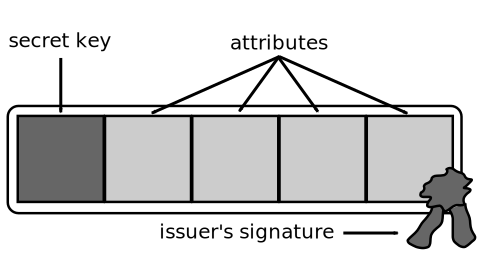
\includegraphics[scale=.45]{images/credential}
  \caption{A first look at an attribute-based credential with four attributes.}
  \label{fig:Credential}
\end{figure}

\subsection{Issuance and Selective Disclosure}

Credentials are \emph{issued} and \emph{verified}, whereas attributes can be
\emph{disclosed} during verification. In the issuance procedure, an issuer and
a user together create a new credential. First the user authenticates to the
issuer in some reliable but unspecified manner (which may be face-to-face). Once
the authentication succeeds, the issuer collects attributes for this user from
trusted databases. The user and issuer then carry out a cryptographic protocol
in which the attributes are combined into a credential signed by the issuer. The
resulting credential contains attributes concerning the user and also his/her
secret key.

The fact that the attributes hold for the owner of a credential is guaranteed
both by the issuer's signature and by the embedded secret key of the owner. The
secret key in the credential is only known by the credential owner and plays an
essential role in verification of the credential. It ensures that a credential
cannot be transferred from one user to another.

A user may have several credentials, each asserting some collection of
attributes. When requesting a service from a service provider, the user is
required to authenticate using one (or more) of his/her credentials. In the
verification process the user can choose to only provide certain credentials;
also, given a specific credential, the user may choose to reveal only a subset
of attributes in the credential. By doing this, authentication becomes more
privacy friendly. This latter process is called selective disclosure, involving
a verification protocol in which only a subset of the credential attributes is
revealed to the verifier while the other attributes are only proved to be
present in the credential. This allows a user to reveal only the necessary
attributes and prove that the credential belongs to him/her. The service
provider can verify all information that has been sent, including the issuer's
signature.

The roles of a service provider and an issuer can also be combined: after
checking one credential, a new one can be issued. For instance, after verifying
an ``over~18'' attribute from an identity credential, a liquor shop might choose
to issue a loyalty credential.

In this paper we stick to a simplistic approach to selective disclosure in which
an index set $\mathcal{D}$ determines the information to be revealed. Selective
disclosure is sometimes defined more generally. We consider only the projection
function $F_{\mathcal{D}}$ that is determined by a disclosing subset
$\mathcal{D}$ of attribute indexes. For example, if there are four attributes
and $\mathcal{D}=\{1,3\}$, then
$F_{\mathcal{D}}(a_1, a_2, a_3, a_4)= (a_1, a_3)$. However, a more general
definition would allow $F$ to be any function of the attributes, for example,
$F(a_1, a_2, a_3, a_4):=(a_1>18, a_2+a_3)$.

\subsection{Security and Privacy}

The cryptographic nature of the credential-as-container concept includes the
following four security aspects.
\begin{itemize}
  \item The issuer's digital signature ensures \emph{authenticity}: the
    credential originates from the issuer, and this issuer asserts that the
    attributes hold for the person.
  \item This signature also guarantees \emph{integrity}: the attributes
    contained in the credential have not been altered since they were issued.
  \item A credential is \emph{non-transferable} as it is bound to the secret
    key of the person involved in the issuance protocol. This secret key should
    be well protected, for instance via storage in the secure memory of a smart
    card with a PIN.
  \item A credential \emph{hides} its content, so it does not reveal the
    attributes it contains.
\end{itemize}
Furthermore, a credential protects the privacy of its owner through the
following cryptographic properties.
\begin{itemize}
  \item \emph{Issuer unlinkability} ensures that any information gathered
    during issuing cannot be used to link a verification of the credential to
    its issuance.
  \item \emph{Multi-show unlinkability} guarantees that when a credential is
    verified multiple times, these sessions cannot be linked.
\end{itemize}
The privacy of users is protected by these unlinkability properties even if the
credential issuer and all verifiers collude. As briefly reviewed below, a
variety of ways of achieving the properties above have been proposed.

\label{unlinkApproaches}
\emph{Blindly signed single-show credentials\footnote{Multi-show unlinkability
for these schemes can be realised by issuing multiple credentials for the same
set of attributes which can later be verified independently.}} are credentials
in which the issuance involves creating a blind signature which conceals the
resulting credential from the issuer. Therefore, the verification instances of
this credential cannot be related to the issuing phase. Examples of this
approach are Brands credentials~\cite{Brands2000}, which are used in
Microsoft's U-Prove system~\cite{U-Prove_Crypto2011}, and Baldimtsi and
Lysyanskaya credentials~\cite{BaLy2012}.

\emph{Randomisable credentials} employ special cryptographic techniques
enabling certain credential structures to be randomised using blinding factors
while preserving their verifiability. In such systems, users can randomise their
credentials before they are verified. Such credentials have been proposed by
Verheul~\cite{Verheul01}, and implemented by Batina et
al.~\cite{BatinaHJMV10}, although this technique currently only supports binary
attributes; for example, instead of a descriptive string of nationality, the
answer to the question ``Is French?'' is stored.

\emph{Zero-knowledge proofs} allow a user to prove ownership of a credential
without revealing the credential itself. Since the verifier does not see the
credential, verification instances are unlinkable and they also cannot be
related to the issuing procedure. Camenisch and
Lysyanskaya~\cite{CL2001,CL2003} combine such proofs with randomisation; their
technique was further developed and became IBM's Identity Mixer
(Idemix)~\cite{idemix_spec_2.3.4}.


-------------------------------------------------------------

A credential is an attestation of qualification, competence, or authority
issued by a third party, the \emph{issuer}, to an individual. This
individual, the \emph{prover}, can subsequently use this credential to
prove\slash demonstrate his qualification, competence, or authority to
another party, the \emph{verifier}. Examples of credentials are a
membership certificate, such as a passport or employee card, or some kind
of ticket to obtain some service, such as a cinema ticket or a public
transport ticket. These credentials are often bound to a specific person,
by means of a name and\slash or picture (e.g.\ for a passport or public
transport year pass), but this is not necessarily the case (e.g.\ for a
paper train ticket).

Anonymous credentials have the same properties as any other credentials,
except that they do not reveal the identity of the prover, i.e.\ they provide
\emph{authorisation without identification}. In the real world this is
fairly common, think of coins or public transport tickets, but in the
digital world this concept is rare. This is mostly because the
authenticity of a credential is usually achieved by using digital
signatures which uniquely identify the issuer and prover. It is however
possible to achieve anonymous digital credentials by using more advanced
cryptography, as described for the first time by Chaum~\cite{Chaum1985} in
1984. In the remainder of this section we will introduce a number of recent
technologies which provide anonymous credentials.

\subsubsection{Self-blindable Credentials}\label{sec:selfblindable}

The idea behind the self-blindable credentials by
Verheul~\cite{Verheul01} is that every time a credential is used it is
blinded such that two occurrences of the same credential cannot be
recognised. This in contrast to the U-Prove token which is the same in
each transaction, and hence serves as a pseudonym. The benefit of this
approach is that the use of such credentials is
untraceable. Furthermore they can be efficiently implemented on a
smart card~\cite{BatinaHJMV10,HoepmanJV10} using elliptic curve
cryptography (ECC), providing the best performance results thus far.

The drawback is that, due to the untraceable nature of this technology,
incorporating revocation is hard and very costly~\cite{HoepmanLV11}.
Furthermore, ECC support on smart cards is very limited making prototyping
very hard. Finally, the technology is fairly new compared to U-Prove and
Idemix, and not backed by a big company which offers support for it.

\subsubsection{U-Prove}\label{sec:uprove}

Stefan Brands provided the first integral description of the U-Prove
technology in his thesis~\cite{Brands2000} in 2000, after which he founded
the company Credentica in 2002 to implement and sell this technology.
Microsoft acquired Credentica in 2008 and published the U-Prove protocol
specification~\cite{U-Prove_Crypto2010} in 2010 under the Open
Specification
Promise\footnote{\url{http://www.microsoft.com/interop/osp/}} together with
open source reference software development kits (SDKs) in C\# and Java.

The U-Prove technology is centred around a so-called U-Prove token. This
token serves as a pseudonym for the prover. It contains a number of
attributes which can be selectively disclosed to a verifier. Hence the
prover decides which attributes to show and which to withhold (e.g.\ one
can reveal the birth date, but not the residence address). Besides the
attributes the token contains two information fields, one defined by the
issuer, and one by the prover. These fields are always disclosed and can be
used to provide some meta data such as a validity date of the token.
Finally there is the token's public-key, which aggregates all information
in the token, and a signature from the issuer over this public-key to
ensure the authenticity.

A previous attempt to implement this technology on a smart card by Tews and
Jacobs~\cite{TewsJacobs09}, based on Brands' description~\cite{Brands2000},
resulted in a highly involved application with running times in the order
of 5--10 seconds which make it not really usable in practice. Our
implementation, which we describe in Section~\ref{sec:uproveimp}, not only
has a much better performance but is also, except from some minimal
limitations, compatible with the development kits released recently by
Microsoft.

U-Prove implementation on a Java Card by Tews and Jacobs~\cite{TewsJacobs09}
U-Prove alternative by Baldimtsi and Lysyanskaya~\cite{BaLy2012}

\subsubsection{Identity Mixer and DAA}\label{sec:idemix}

Identity mixer (Idemix) is an anonymous credential system, based on the
Camenisch-Lysyanskaya anonymous credentials
scheme~\cite{CamenischLysyanskaya2001, CamenischLysyanskaya2002,
Lysyanskaya2002} developed at IBM Research in Z\"urich that enables strong
authentication and privacy at the same time. The first
prototype~\cite{CamenischH02} was developed in 2002 and has been improved
over the years. An open source Java implementation of Idemix was released
in 2010 as part of the Open Innovation
Initiative.\footnote{\url{http://www.zurich.ibm.com/news/10/innovation.html}}

Direct anonymous attestation (DAA)~\cite{BrickellCC04} is a technology based
on Idemix. It allows a user to convince a verifier that she uses a platform
that has embedded a certified hardware module.\footnote{DAA has
been adopted in 2004 by the Trusted Computing Group in the Trusted Platform Module
specification as the method for remote authentication of a hardware
module.} The protocol protects the user's privacy: if she talks to the same
verifier twice, the verifier is not able to tell whether or not he
communicates with the same user as before or with a different one.

In 2009 Bichsel et al.~\cite{BichselCGS2009} implemented Idemix on a Java
Card whereas Sterckx et al.~\cite{Sterckx09} did the same for DAA. They
provide the first proper implementations of anonymous credentials on smart
cards. The major drawback of these implementations is the running
time of several seconds which is still too much for being really practical.

Idemix is used for Direct Anonymous Attestation~\cite{BrickellCC2004} in the TPM
specification~\cite{TPM}.
Idemix implementation on Java Card by Danes~\cite{Danes}, IBM Bichsel et al.~\cite{BichselCGS2009}, Sterckx et al.~\cite{Sterckx09}

ABC4Trust

\subsubsection{German Identity Card}

The protocols that we have described so far are (to the best of our
knowledge) the only candidates providing anonymity by design and ones
that \emph{could} be implemented on a smart card. However, we should
also shortly mention an approach of the German identity card that is
actually implemented and being rolled out since November 2010, where a
limited form of anonymous attribute use is achieved by altering the
existing ECC based electronic identity protocols by sharing private ECC
keys across large batches of cards~\cite{Kugler2010}. The protocol itself
provides restricted access to the card by means of the so-called
card verifiable certificate mechanism~\cite{EAC20} and
allows for selective disclosure of attributes, depending on the rights
specified in the certificate (e.g.\ an alcohol shop is only authorised to check for
the ``over~18'' attribute). Signed attributes are partly anonymous
because of the sharing of the signing keys between batches of cards, such
that a signature cannot be linked to a single card.

\section{Smart Cards}

One of the goals of our research is to assess
how fast privacy-friendly protocols are when run on a smart card.
Hence implementing our prototypes requires an open smart card
platform that also provides the necessary cryptographic hardware
support -- previous research~\cite{TewsJacobs09} clearly shows
that, in terms of performance, purely software based prototypes are
not sufficient for realistic use. In practice that leaves us with
two possible smart card platforms, Java Card and MULTOS, described
below. We motivate the use of the latter one for the work presented
in this paper.

Regardless of the programming technology, all smart cards provide the
same external functionality. A smart card is an embedded device that
communicates with the environment through Application Protocol Data
Units (APDUs) -- byte arrays formatted according to the ISO7816
specification.  Most notably, the APDUs constrain the communication
payload to roughly 256 bytes in each direction for a single APDU exchange.
The permanent storage
of the card (EEPROM memory) is considered highly secure, accessible
only through the APDU commands offered by the application, which in
turn are subject to any authentication and secure messaging
requirements that the card application may impose.

Regardless of the software platform operating the card, all smart cards provide
the same external functionality. A smart card is an embedded device that
communicates with the environment through Application Protocol Data Units
(APDUs) -- byte arrays formatted according to the ISO7816
specification~\cite{ISO7816_4}. Most notably, the APDUs constrain the
communication payload to roughly 256 bytes in each direction for a single APDU
exchange. The permanent storage of the card (EEPROM memory) is considered
highly secure, accessible only through the APDU commands offered by the
application, which in turn are subject to any authentication and secure
messaging requirements that the card application may impose.

\subsubsection{Java Card}\label{sec:javacard}

Java Card is a now well-established smart card platform based on a
tailored, cut-down version of Java (hence the name)~\cite{Chen00}. One
of the main features of Java Card is software interoperability. On top
of the operating system of the card resides a Java Card virtual
machine, compliant with the official specification~\cite{jcvm222}, that
executes Java byte code. In parallel, the platform defines
the Java Card API~\cite{jcapi222} that provides the developer an interface
to the hardware of the smart card.
In terms of the programming and deployment of applications
Java Cards are (almost) fully independent of the underlying hardware
and operating system of the card. Large numbers of actual smart card
products are implemented on Java Cards based on a variety of chips
coming from different manufactures. Precise data on the number of deployed
Java Cards or MULTOS cards are hard to find, but the
Java Card Forum\footnote{\url{http://www.javacardforum.org/}}
claims there are already over a billion Java Cards in use.

%%% Old url: http://www.embeddedstar.com/press/content/2004/11/embedded17020.html

The Java Card API is carefully designed to support the smart card
environment and has several built-in security features. For example,
it provides predefined Java classes for hardware supported
cryptographic key storage (with possible internal encryption). To
account for different hardware profiles of a card, parts of the Java
Card API implementation are made optional. For example, one card may
support both RSA and ECC in hardware and expose this functionality
through the API, while another card may only support RSA, in which
case all API calls related to ECC are not available and report a
corresponding Java exception instead.

This brings us to the main shortcoming of the Java Card platform from our
point of view. The Java Card API is predefined
and \emph{closed}. Any hardware functionality that is not exposed
through the imposed Java Card API, is not accessible to the developer
by any other means. For example, for RSA based cryptography it is only
possible to generate public and private keys of predefined RSA lengths
(512, 1024 bits, etc.) and perform full RSA de-/encryption or signing
with these keys according to standard protocols, such as RSA-PKCS.  The
more primitive operations that build up RSA operations, such as modulo
prime inverse or exponentiation, are not available. Since all of the
protocols that we are interested in require access to such cryptographic operations
(in large modulo prime and/or EC domains), this is a practical show
stopper. We are not the only ones to note this. For example,
in~\cite{Sterckx09}
similar problems regarding the development of DAA on a Java Card are
reported.  Even more, an efficient implementation of the e-passport
standard~\cite{EAC20} on a Java Card also requires cryptographic
routines not anticipated by the standard Java Card API. In this case,
due to high demand, Java Card producers decided to enrich the Java
Card API with proprietary extensions to support e-passport
standards~\cite{NXP09}. But this only solves the problem for one
application type and, moreover, makes the platform non-interoperable.

\subsubsection{MULTOS}\label{sec:multos}

The design principles of the MULTOS
platform~\cite{MULTOS2005,MULTOS_Manual2009} are similar to those of
Java Card. A hardware independent execution platform is run on top of
the operating system of the card. Similarly to Java Card byte-code, a
MULTOS card executes specific op-codes of the MULTOS Execution
Language (MEL) and exposes smart card specific interfaces to the
developers through dedicated MEL op-codes. These
op-codes already provide a full and detailed API to the card's
hardware. Most of the primitive operations that the hardware can
possibly support are reflected in the corresponding MEL
op-codes. Thus, MEL provides the full base for programming MULTOS
cards, and a skilled developer can easily write programs for the
card already in the MEL assembly. However, the MULTOS development
tools also provide programming interfaces to C and Java. Applications
in these languages are translated\slash compiled by the tools into MEL op-codes and
can then be run on a card.

Similar to the Java Card API routines, some of the MEL op-codes are
specified to be optional, mostly ones responsible for cryptographic
operations. A particular MULTOS card may or
may not support the optional op-codes. For our implementation we used
development cards based on the SLE66 chip from Infineon. This particular
MULTOS implementation~\cite{MULTOS_Implementation2010} supports a wide
range of modulo arithmetic operations, a range which is sufficient
to fully support all of the U-Prove calculations.
This is the main reason to choose MULTOS in the context of this work --
its more low-level and flexible API as opposed to less flexible
and more high level Java Card API.

%%% A link with some MULTOS data, just in case:
%%% http://www.cts-caliber.com/products_SMC01.html

Our choice is to use the MULTOS C interface to do our prototype
implementation of U-Prove. For simple smart card applications the C
interface seems to provide an easier programming environment than
Java, and although C programming platforms are not type safe by
definition (as opposed to Java), per application memory safety is
guaranteed by the MULTOS platform, regardless of the high-level language
used during development.

The goal of the MULTOS platform is to provide a secure hardware independent
execution platform for smart cards. To this end, they developed a specification
for the execution and memory models, explained in more detail below, that all
MULTOS implementations must provide. Besides this mandatory part of the
specification there are also a number of optional elements, mostly concerning
cryptographic functionality that may or may not be available on a specific
hardware platform. An overview of which functionality is provided by which card
can be found in the MULTOS Implementation Reference~\cite{MIR2012}\footnote{Our
card has an M3 generic (ML3-36K-R1) implementation by Multos International.}.

\subsubsection{Execution Model}

Applications on a MULTOS card are executed in a virtual machine, called the
Application Abstract Machine (AAM). The functionality of this virtual machine
is defined by the MULTOS specification to assure that applications are
portable, that is, independent of the actual chip used\footnote{Application
portability can be limited due to specific memory requirements or dependencies
on optional parts of the MULTOS specification.}. The AAM is a stack machine
that interprets instructions from the MULTOS Executable Language (MEL).

\subsubsection{Memory Model}

The AAM virtual machine provides each application with its own memory space.
Within an application the code space, residing on non-volatile EEPROM storage,
and data space, divided over EEPROM (for persistent storage) and volatile RAM,
are handled independently of each other. Code is executed while data is
manipulated. The memory of an application is protected by a strong firewall.
This means that applications cannot access each others memory. The data of
an
application is divided over three distinct memory areas, listed below.

\paragraph{Static memory} is the non-volatile storage for an application. It is
private to the application and cannot be accessed by the terminal or any other
application. MULTOS offers mechanisms to avoid corruption of the static memory
area such that this data remains consistent.

\paragraph{Public memory} is the volatile input/output buffer for an
application. Incoming command APDUs are held in public memory and outgoing
response APDUs are placed here. This buffer is also used to pass information
from one application to another when delegation is used. MULTOS guarantees that
data in this memory remains private to the running application until it exits
or delegates to another application. This means that it can be used as
temporary workspace.

\paragraph{Dynamic memory} is the volatile storage for an application. It is
used to store session data, if any. The size of the session data area is fixed
when an application is loaded onto a card and it depends on the amount of
variables declared. Furthermore, the dynamic memory contains the stack, which
is the application's work area. As mentioned before, the AAM operates as a
stack machine, which means that this memory area is used to perform many
functions (and provide input for these functions). The maximum size of the
stack is fixed by the amount of dynamic memory available. Therefore,
applications will need to ensure that their use of dynamic memory does not
exceed the limit imposed by the chip~\cite{MIR2012} on which the application
will reside.


\section{Contributions}

All contributions are available as open source software under the GNU General
Public License\footnote{\url{https://www.gnu.org/copyleft/gpl.html}}, version~3.

\subsection{Self-blindable Credentials}

The third chapter is based on two papers, \emph{Developing Efficient Blinded
Attribute Certificates on Smart Cards via Pairings}~\cite{BatinaHJMV10} which
is joint work with Lejla Batina, Jaap-Henk Hoepman, Bart Jacobs and Wojciech
Mostowski, and \emph{Privacy and Security Issues in e-Ticketing -- Optimisation
of Smart Card-based Attribute-proving}~\cite{HoepmanJV10} which is joint work
with Jaap-Henk Hoepman and Bart Jacobs. I presented this work at the 9th IFIP WG
8.8/11.2 International Conference on Smart Card Research and Advanced
Applications (CARDIS 2010).

\paragraph{Contribution}

My contribution in this chapter is the development and analysis of the efficient
smart card implementation of the self-blindable credentials technology as well
as the implementation of the corresponding host software. This consists of:
\begin{itemize}
  \item the Java Card applet\footnote{\url{https://github.com/pimvullers/sbcred_javacard/}},
    which provides the cryptographic operations on the smart card;
  \item the terminal software\footnote{\url{https://github.com/pimvullers/sbcred_terminal/}},
    which provides the cryptographic operations for the issuer and verifier as
    well as the protocol interaction with the smart card; and
  \item an extension\footnote{\url{https://github.com/pimvullers/bouncycastle-ext/}}
    to the Bouncy Castle cryptographic library\footnote{\url{http://bouncycastle.org/java.html}},
    which adds support for elliptic curve bilinear pairings.
\end{itemize}

\subsection{U-Prove}

The fourth chapter is based on the paper \emph{Efficient U-Prove Implementation
for Anonymous Credentials on Smart Cards}~\cite{MostowskiVullers11} which is
joint work with Wojciech Mostowski. I presented this work at the 7th
International ICST Conference on Security and Privacy in Communication Networks
(SecureComm 2011).

\paragraph{Contribution}

My contribution in this chapter is the analysis of the efficient smart card
implementation of the U-Prove technology as well as the development of the
terminal software\footnote{\url{https://github.com/pimvullers/uprove_terminal/}}
which builds upon the U-Prove SDK\footnote{\url{http://archive.msdn.microsoft.com/uprovesdkjava/}}
and takes care of the protocol interaction with the smart card. Furthermore I
provided the pseudo code that allowed my co-author to develop the MULTOS
application\footnote{\url{https://github.com/pimvullers/uprove_multos/}} which
provides the cryptographic operations on the smart card.

\subsection{Identity Mixer}

The fifth chapter is based on the paper \emph{Efficient Selective Disclosure on
Smart Cards using Idemix}~\cite{VullersAlpar2013} which is joint work with
Gergely Alp\'ar. I presented this work at the 3rd IFIP WG 11.6 Working
Conference on Policies and Research in Identity Management (IDMAN 2013).

\paragraph{Contribution}

My contribution in this chapter is the development and analysis of the efficient
smart card implementation of the Identity Mixer technology as well as the
implementation of the corresponding host software. This consists of:
\begin{itemize}
  \item the MULTOS application\footnote{\url{https://github.com/pimvullers/idemix_multos/}
    }\footnote{This has evolved into the IRMA application
    (\url{https://github.com/pimvullers/irma_card/}) which provides additional
    functionality, like secure messaging and an interface which allows the user
    to manage the credentials stored on the card.}
    which provides the cryptographic operations on the card; and
  \item the terminal software\footnote{\url{https://github.com/pimvullers/idemix_terminal/}}
    which provides the protocol interaction between the smart card and our
    patched version\footnote{\url{https://github.com/pimvullers/idemix_library/}}
    of the Identity Mixer cryptographic library\footnote{\url{https://prime.inf.tu-dresden.de/idemix/}}.
\end{itemize}

With this implementation I laid out the foundations % Alternatief: paved the way
for the IRMA project\footnote{\url{https://irmacard.org/}}. This is an on-going
research and development project focussing on attribute-based credentials and
their use in practice.